%************************************************
%\chapter{Distinction of drivers in pCO$_2$} % $\mathbb{ZNR}$
\chapter{Contribution of different processes to multi-year pCO$_2$ trends} % $\mathbb{ZNR}$
%
%************************************************
\label{ch:pCO2separation}

%\paragraph{Purpose of pCO$_2$ separation}
%\subsection{Explanation and assuof the framework and its assumptions}
The previous analysis of thermal, physical and biological controls of the Southern Ocean carbon sink asks for an estimate on the relative contributions of each process to the total change. As interconnected processes always influence and change each other directly, a clear and clean separation cannot be taken in precision, but rather as an \textit{estimate of the first-order drivers} in CO$_2$ flux. In this chapter, I adapt the pCO$_2$ diagnostics framework from \cite{Lovenduski2007} to quantitatively relate the different contributors to pCO$_{\text{2,ocean}}$ and hence CO$_2$ flux.

\section{Derivation of the framework}
The framework assumes an euphotic zone zonal carbon budget box, where \acs{DIC} enters at the upper boundary  via CO$_2$ flux and \acs{DIC} leaves the system at the lower boundary at the \acs{MLD} as biology export production  (fig. \ref{fig:pCO2_separation}). Based on the individual processes taking place, a change in pCO$_2$ due to that process is calculated offline, i.e. from monthly model output data, instead of online, i.e. for each timestep when the model ran. Also the carbonate chemistry and the changes in pCO$_2$ related to changes in \acs{DIC} and alkalinity are calculated monthly. \newline

\begin{figure}[h!]
	\centering
	\includegraphics[scale=.51,page=2,trim=5.cm 4.7cm 2.7cm 1.3cm,clip]{co2sep}
	\caption{Schematic illustration of pCO$_2$ driver separation assuming a well-mixed zonal carbon box of the upper-ocean, where CO$_2$ flux (red) is separated in contributions due to thermal (orange), freshwater (light blue), biology (green) and a residual for circulation (dark blue)}	
	\label{fig:pCO2_separation}
\end{figure}

I separate pCO$_2$ into contributions of temperature, salt, alkalinity and DIC. I use the salinity-normalized concentrations $(sDIC=\frac{DIC}{S}\cdot (S_0=35))$ for DIC and alkalinity to prevent double-accounting of freshwater changes in the DIC/alkalinity and salt contributions \citep{Keeling2004}.

\begin{align*}
\delta pCO_2&=\delta pCO_{\text{2,thermal}}+\delta pCO_{\text{2,salt}}+\delta pCO_{\text{2,alk}}+\delta pCO_{\text{2,DIC}} \\ \\
&= \frac{\partial pCO_2}{\partial T}\delta T + \frac{\partial pCO_2}{\partial S}\delta S  + \frac{S}{S_0}\frac{\partial pCO_2}{\partial Alk}\delta sAlk  \\ &+ \frac{S}{S_0}\frac{\partial pCO_2}{\partial DIC}\delta sDIC + \frac{\partial pCO_2}{\partial FW}\delta FW 
\end{align*}

\noindent The thermal separation is taken from \cite{Takahashi1993}:
\begin{align*}
\frac{\partial pCO_2}{\partial T} &\approx \overline{pCO_2} \cdot 0.0423 ^\circ C^{-1}  .
\end{align*}

\noindent The salinity, DIC and alkalinity contributions are taken from \cite{Sarmiento2006}:
\begin{align*}
\allowdisplaybreaks
\frac{\partial pCO_2}{\partial S} &\approx \frac{pCO_2}{S} \cdot \gamma_{S}  \\
\frac{\partial pCO_2}{\partial DIC} &\approx \frac{pCO_2}{DIC} \cdot \gamma_{DIC} \\
\frac{\partial pCO_2}{\partial Alk} &\approx \frac{pCO_2}{Alk} \cdot \gamma_{Alk} \\
\frac{\partial pCO_2}{\partial FW} &\approx \frac{pCO_2}{MLD} \cdot \gamma_{FW} \\
\gamma_{DIC} &\approx \frac{3 \cdot Alk \cdot DIC - 2 \cdot DIC^2}{(2 \cdot DIC - Alk)(Alk-DIC)} \\
\gamma_{Alk} &\approx -\frac{Alk^2}{(2 \cdot DIC - Alk)(Alk-DIC)} \\
\gamma_{S} &\approx 1 \\
\gamma_{FW}&=\gamma_{Alk}+\gamma_{DIC}+\gamma_{S}.
\end{align*}

\noindent Furthermore the changes in sDIC and sAlk are separated into biological, sea-air exchange or residual contribution to check for the origin of \acs{DIC} changes, \ie biological export, CO$_2$ flux or other not specified processes such as upwelling or lateral transports:

\[\frac{\delta (sDIC)}{\delta t}=\frac{\delta (DIC_{bio})}{\delta t}+\frac{\delta (DIC_{exchange})}{\delta t}+\frac{\delta (sDIC_{res})}{\delta t}.\]

\noindent The changes due to sea-air exchange and due to biology are converted to \acs{DIC} and alkalinity changes by dividing by the \ac{MLD} assumping a well-mixed \acs{MLD}. Furthermore, the effect of biological primary production contributes with organic matter production (coex) and calcium carbonate (caex) production to changes in DIC and alkalinity.
\begin{align*}
\delta DIC_{bio}&=-\frac{coex+caex}{MLD} \\
\delta DIC_{ex}&=-\frac{CO_2flux}{MLD} \\
\delta Alk_{bio}&=-\frac{2caex-16/122 \cdot coex}{MLD}
\end{align*}

\vspace{1cm}

This approach is based on the following assumptions:
\begin{itemize}
\item[-] negligible errors in approximations used during derivation
\item[-] linearizations of non-linear processes
\item[-] steady state over timestep of calculation, \eg one month
\item[-] simplifications of buffering constants \citep{Sarmiento2006}
\item[-] residual as combined contribution of everything which is not described, mainly vertical and lateral circulation, but also to a lesser degree advection of biological constituents
\item[-] ignoring time-averaging inconsistency: monthly mean offline instead of instantaneous online calculation
\item[-] well-mixed mixed layer
\end{itemize}

\clearpage
\section{Estimate of pCO$_2$ drivers}


Applying the above described framework yields an estimate for the drivers of pCO$_2$ for the two extreme trends (table \ref{tab:trends_pco2}).

\begin{table}[h!]
\centering
\begin{tabular}{ l | c c | c c}
\multicolumn{5}{l} {8-yr trend} {\hspace{1.cm} 50-60$^\circ$S \hspace{2.cm} 40-50$^\circ$S} \hspace{1.cm} \\ \hline
%{8-yr trend} \multicolumn{2}{l} 50-60$^\circ$S \multicolumn{2}{l} 40-50$^\circ$S} \\ \hline
  pCO$_{\text{2,x}}$  [ppm] & positive  & negative & positive  & negative  \\
  \hline  

  pCO$_{\text{2,freshwater}}$ & 0.6 & -0.5 & 0.2 & -0.3 \\
  pCO$_{\text{2,salt}}$ & 0.6 & -0.5 & 0.2 & -0.3 \\
  pCO$_{\text{2,sDIC}}$ & 37.6 & 1.0 & -2.3 & 19.1 \\
  pCO$_{\text{2,sAlk}}$ & 8.1 & -4.2 & -1.8 & -1.5 \\
  \hline  
  pCO$_{\text{2,ex,dic}}$ & -5.1 & 5.2 & 0.2 & 1.1 \\
  pCO$_{\text{2,bio,dic}}$ & 2.7 & -3.4 & -0.8 & -0.2 \\
  pCO$_{\text{2,bio,alk}}$ & 0.3 & -0.3 & -0.1 & -0.0 \\
  pCO$_{\text{2,res,sDIC}}$ & 40.0 & -0.8 & 9.8 & 18.2  \\
  pCO$_{\text{2,res,sAlk}}$ & 7.8 & -3.9 & -1.7 & -1.5 \\
  \hline  
  pCO$_{\text{2,non-thermal}}$ & 38.2 & -8.3 & 3.4 & 12.0  \\
  pCO$_{\text{2,thermal}}$ & -7.1 & 7.0 & 6.4 &  0.5 \\  
  \hline
  pCO$_{\text{2,ocean}}$ & 32.2 & -2.4 & 9.4 &  12.9 \\
  pCO$_{\text{2,atm}}$ & 12.0 & 14.5 & 12.0 &  14.5 \\
  \hline \hline
  dpCO$_{\text{2}}$ & 20.2 & -16.9 & -2.6 & -1.6  \\
\end{tabular}
\caption{Trends in drivers of pCO$_2$ for the most extreme positive CO$_2$ flux trend and the most most extreme negative CO$_2$ flux trend in two 10$^\circ$-\ac{MLD} boxes}
\label{tab:trends_pco2}
\end{table}

In broad terms, the trends reverse for opposite wind forcing and the area 50-60$^\circ$S sets the trend of the overall Southern Ocean carbon sink south of 35$^\circ$S. The change in sDIC and sAlk dominate over the thermal, dilution and saline effect. The changes in pCO$_2$ due to biology and temperature are much smaller than the residual change. So, the major contributor to the pCO$_2$ is neither biology nor temperature, but not directly accounted for. Most likely changes in ocean circulation account for this residual and therefore highly depend on the history of the water masses which enter my box of interest. Here, the sDIC contribution dominates over the sAlk contribution (expect for negative trend at 50-60$^\circ$S).%note on seasonality

Overall, biology seems more susceptible to wind-driven changes at 50-60$^\circ$S than 40-50$^\circ$S, this separation might be biased by the selection of the latitudinal boundaries.\newline

In detail, the ongoing processes do not simply reverse as the atmospheric forcing trend stays the same. 
The most positive CO$_2$ flux trend is mainly driven by the non-thermal pCO$_{\text{2,ocean}}$ ocean changes, whereas the most negative CO$_2$ flux trend is mainly driven by the increasing pCO$_{\text{2,atm}}$ concentrations, when the oceanic pCO$_{\text{2,ocean}}$ only has a very weak uptake trend and the upper-ocean overturning cell shifts northward.

In the negative CO$_2$ flux trend, pCO$_{\text{2,ocean}}$ due to circulation increases at 40-50$^\circ$S, whereas less Ekman transport would predict a decrease. Here for the northward shift of the westerlies, the upwelling cell migrated northwards and thus increased the entrainment of carbon-rich waters. Also the warming extends further north into the area of 40-50$^\circ$S, which shifts the increasing pCO$_{\text{2,ocean}}$ trend from cooling out of 40-50$^\circ$S, resulting in a positive thermal trend.




%\clearpage

%\subsection{Interplay of processes}

%\paragraph{positive CO$_2$ flux trend}
\label{sec:pCO2separation_pos}

Combining the three distinct pCO$_2$ responses for the most extreme positive CO$_2$ flux trend from section \ref{sec:trends_pos} leads to a comprehensive picture (fig. \ref{fig:schematics_pos}). 
While the cooling effect of the stronger winds reduces outgassing in the high-latitude Southern Ocean, the increase in upwelling of carbon-rich waters and the decline in primary production outplay the thermal effect to a relative outgassing trend at 50-60$^\circ$S. At 40-50$^\circ$S the warming effect and  increased Ekman transport DIC supply reduces carbon uptake, which is overtrumped by increase primary production and increased downwelling and leads to a combined relative CO$_2$ uptake trend. The resulting CO$_2$ flux signal at 50-60$^\circ$S is stronger than the one at 40-50$^\circ$S and hence determines the overall Southern Ocean carbon sink trend. The overall positive CO$_2$ flux trend and its opposite thermal contribution is in line with \cite{Lovenduski2007}.\newline


\begin{figure}[h!]
	\centering
	\includegraphics[scale=.5,trim=4.cm 1.5cm 2cm 0cm,clip,page=17]{SO_schematics}
	\caption{Schematic illustration of the Southern Ocean under the context of increasing westerly winds and response in the thermal effect, biology and upper-ocean circulation leading towards a positive CO$_2$ flux trend; red color-coding indicates a relative increase of the related quantity or process whereas blue indicates a relative decrease. Stronger winds enhance the upper-ocean overturning circulation. Increased upwelling increases outgassing of over-saturated carbon-rich deep waters. Increased Ekman transport advects DIC further north, cools the higher latitudes whereas it warms the lower latitudes. Deeper mixing and cooling in the higher latitudes decreases primary production whereas shallower mixing and warming increase primary production in the higher latitudes.}
	\label{fig:schematics_pos}
\end{figure}



\clearpage
%\paragraph{negative CO$_2$ flux trend}
\label{sec:pCO2separation_neg}
The three distinct pCO$_2$ responses for the most extreme negative CO$_2$ flux trend from section \ref{sec:trends_neg} merge into the opposing picture as for decreasing westerly winds (fig. \ref{fig:schematics_neg}). 
While the warming effect of the weaker winds increases outgassing in the high-latitude Southern Ocean, the decrease in upwelling of carbon-rich waters and the decline in primary production outplay the thermal effect to a relative ingassing trend at 50-60$^\circ$S. At 40-50$^\circ$S the cooling effect and decreased Ekman transport DIC supply relatively increase carbon uptake, which is overtrumped by decreased primary production and decreased downwelling and leads to a combined relative CO$_2$ outgassing trend. The resulting CO$_2$ flux signal at 50-60$^\circ$S is stronger than the one at 40-50$^\circ$S and hence determines the overall Southern Ocean carbon sink trend.


\begin{figure}[h!]
	\centering
	\includegraphics[scale=.5,trim=4.cm 1.5cm 2cm 0cm,clip,page=18]{SO_schematics}
	\caption{Schematic illustration of the Southern Ocean under the context of decreasing westerly winds and response in the thermal effect, biology and upper-ocean circulation leading towards a negative CO$_2$ flux trend; red color-coding indicates a relative increase of the related quantity or process, whereas blue indicates a relative decrease. Stronger winds decrease the upper-ocean overturning circulation. Decreased upwelling lowers outgassing of over-saturated carbon-rich deep waters. Decreased Ekman transport advects less DIC to the north, warms the higher latitudes whereas it cools the lower latitudes. Shallower mixing and warming in the higher latitudes increases primary production, whereas deeper mixing and cooling decrease primary production in the higher latitudes.}
	\label{fig:schematics_neg}
\end{figure}
